% =========
% CHƯƠNG 5
% =========
\OpenGrid

\ParallelChapter
  {Reasoning with Algebraic Symbols}
  {Luận với kí hiệu đại số}
  {}

\TriPara
  {
    \EN{The algebraic notation we use today is a major accomplishment of humankind, allowing for the compact representation of complex calculations and problems (Fey 1984; Radford and Puig 2007). However, that very compactness can be a barrier to sense making (Radford and Puig 2007; Saul 2001). A basic task for teachers of algebra is to help students reason their way through that barrier.}
  }
  {
    \VI{Kí hiệu đại số mà ta sử dụng ngày nay là một thành tựu lớn của nhân loại, cho phép biểu diễn gọn gàng những phép tính và bài toán phức tạp (Fey 1984; Radford and Puig 2007). Tuy nhiên, chính sự cô đọng đó đôi khi lại trở thành rào cản đối với hiểu (Radford and Puig 2007; Saul 2001). Một nhiệm vụ cơ bản của giáo viên đại số là giúp học sinh luận để vượt qua rào cản ấy.}
  }{\NOTE{}}

\TriPara
  {
    \EN{Key elements of reasoning and sense making with algebraic symbols include the following:

    \begin{itemize}
      \item \emph{Meaningful use of symbols.} Choosing variables and constructing expressions and equations in context; interpreting the form of expressions and equations; manipulating expressions so that interesting interpretations can be made.
      
      \item \emph{Mindful manipulation.} Connecting manipulation with the laws of arithmetic; anticipating the results of manipulations; choosing procedures purposefully in context; picturing calculations mentally.
      
      \item \emph{Reasoned solving.} Seeing solution steps as logical deductions about equality; interpreting solutions in context.
      
      \item \emph{Connecting algebra with geometry.} Representing geometric situations algebraically and algebraic situations geometrically; using connections in solving problems.
      
      \item \emph{Linking expressions and functions.} Using multiple algebraic representations to understand functions; working with function notation.
    \end{itemize}

    We address these key elements in more detail in the following sections.}
  }
  {
    \VI{Các yếu tố then chốt của luận và hiểu với kí hiệu đại số gồm có:
    \begin{itemize}
      \item \emph{Sử dụng kí hiệu có nghĩa.} Chọn biến và lập biểu thức, phương trình trong ngữ cảnh; diễn giải dạng của biểu thức và phương trình; biến đổi biểu thức để có thể đưa ra những diễn giải đáng chú ý.\vspace{\baselineskip}

      \item \emph{Biến đổi có ý thức.} Gắn việc biến đổi với các luật số học; dự đoán kết quả của phép biến đổi; lựa chọn thủ tục có chủ đích trong ngữ cảnh; hình dung phép tính trong đầu.\vspace{\baselineskip}

      \item \emph{Giải có cơ sở luận.} Nhìn nhận các bước giải như những suy diễn logic về quan hệ bằng nhau; diễn giải nghiệm trong ngữ cảnh.

      \item \emph{Kết nối đại số với hình học.} Biểu diễn tình huống hình học bằng đại số và tình huống đại số bằng hình học; sử dụng các kết nối đó trong giải quyết vấn đề.
      
      \item \emph{Liên kết biểu thức và hàm số.} Sử dụng nhiều dạng biểu diễn đại số để hiểu hàm số; làm việc với kí hiệu hàm.
    \end{itemize}

    Chúng tôi sẽ xử lí chi tiết hơn các yếu tố then chốt này trong các phần tiếp theo.}
  }{\NOTE{}}

\ParallelSection
  {Meaningful Use of Symbols}
  {Sử dụng kí hiệu có nghĩa}
  {}

\TriPara
  {
    \EN{Meaningful use of symbols includes carefully defining the meaning of symbols introduced to solve problems, including specifying units and distinguishing among the three main uses of variables---(1) as unknowns (e.g., find the value of $Q$ such that $3Q - 4 = 11$), (2) as placeholders that can take on a range of values (e.g., $a + c = c + a$ for all $a$ and $c$), and (3) as parameters of a function (e.g., What is the effect of increasing m on the graph of $y = mx + b$?) (Usiskin 1988).}
  }
  {
    \VI{Sử dụng kí hiệu có nghĩa bao gồm việc xác định rõ ràng ý nghĩa của kí hiệu được đưa vào để giải quyết vấn đề, trong đó có việc chỉ rõ đơn vị đo và phân biệt ba cách sử dụng chính của biến---(1) như ẩn số (ví dụ, tìm giá trị của $Q$ sao cho $3Q - 4 = 11$); (2) như kí hiệu giữ chỗ có thể nhận một dải giá trị (ví dụ: $a + c = c + a$ với mọi $a$ và $c$); (3) như tham số của một hàm số (ví dụ, việc tăng $m$ tác động thế nào đến đồ thị của hàm $y = mx + b$?) (Usiskin 1988).}
  }
  {
    \NOTE{\noindent Có ba vai trò chính của biến: 

    \begin{itemize}
      \item biến-ẩn số,
      \item biến-giữ chỗ,
      \item biến-tham số.
    \end{itemize}
    }
  }

\TriPara
  {
    \EN{Although a long-term goal of algebraic learning is a fluid, nearly automatic facility with manipulating algebraic expressions that might seem to resemble what is often called ``mindless manipulation,'' this ease can best be achieved by first learning to pay close attention to interpreting expressions, both at a formal level and as statements about real-world situations. At the outset, the reasons and justifi cations for forming and manipulating expressions should be major emphases of instruction (Kaput, Blanton, and Moreno 2008). As comfort with expressions grows, constructing and interpreting them require less and less effort and gradually become almost subconscious. The true foundation for algebraic manipulation is close attention to meaning and structure.}
  }
  {
    \VI{Mặc dù mục tiêu dài hạn của việc học đại số là hình thành khả năng biến đổi biểu thức đại số một cách trôi chảy, gần như tự động---điều thoạt nhìn có thể giống với cái thường được gọi là ``biến đổi máy móc''---sự thành thạo ấy được đạt đến tốt nhất bằng cách trước hết học cách chú ý kĩ đến việc diễn giải biểu thức, cả trên bình diện hình thức lẫn như những phát biểu về tình huống trong thế giới thực. Ở giai đoạn đầu, lí do và biện minh cho việc lập và biến đổi biểu thức cần là những trọng tâm lớn của dạy học (Kaput, Blanton, and Moreno 2008). Khi mức độ quen thuộc với biểu thức tăng lên, việc lập và diễn giải chúng đòi hỏi ngày càng ít công sức hơn và dần trở nên gần như dưới ngưỡng ý thức. Nền tảng thực sự của biến đổi đại số là sự chú ý sát sao đến ý nghĩa và cấu trúc.}
  }{\NOTE{}}


\TriPara
  {
    \EN{Reasoning with algebraic expressions depends on being able to read them in different ways, for example, seeing $3 - (4 - x)^2$ as 3 minus a quantity squared and thus as a value less than or equal to 3, as a function of $4 - x$, and as a function of $x$. In example 5 students are asked to interpret the purposes of different forms of the same expression.}
  }
  {
    \VI{Luận với biểu thức đại số phụ thuộc vào khả năng đọc biểu thức theo nhiều cách khác nhau. Chẳng hạn, biểu thức $3 - (4 - x)^2$ có thể được nhìn như $3$ trừ đi bình phương của một đại lượng, từ đó thấy rằng giá trị của nó luôn nhỏ hơn hoặc bằng $3$; đồng thời có thể được nhìn như một hàm của đại lượng $4 - x$, và cũng như một hàm của $x$. Trong Ví dụ 5, học sinh được yêu cầu diễn giải tác dụng của những dạng khác nhau của cùng một biểu thức.}
  }{\NOTE{}}

\TriExample
  {Horeshoes in Flight}
  {
    \textbf{Task}

    The height of a thrown horseshoe depends on the time that has elapsed since its release, as shown in the graph. Note that this graph is parabolic, but it may not be the same as the graph of the horseshoe's path. Its height (measured in feet) as a function of time (measured in seconds) from the instant of release is
    $$
      1\frac{3}{16}+18t-16t^2.
    $$

    \begin{center}
      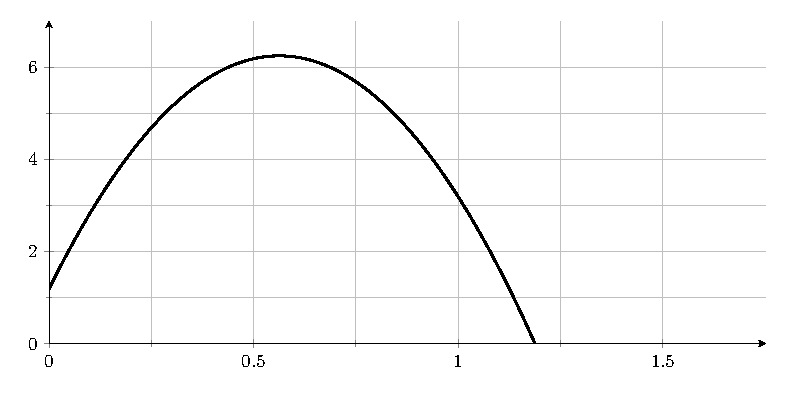
\includegraphics[width=.92\linewidth]{../figures/fhsm_2009_p32_1.pdf}
    \end{center}\vspace{.25\baselineskip}

    The expressions (a)--(d) below are equivalent. Which is most useful for finding the maximum height of the horseshoe, and why is it the most useful expression?

    \begin{description}
      \item [\normalfont (a)] $1\frac{3}{16}+18t-16t^2$
      
      \item [\normalfont (b)] $-16\left(t-\frac{19}{16}\right)\left(t+\frac{1}{16}\right)$
      
      \item [\normalfont (c)] $\frac{1}{16}\left(19-16t\right)\left(16t+1\right)$
      
      \item [\normalfont (d)] $-16\left(t-\frac{19}{16}\right)^2+\frac{100}{16}$
    \end{description}

    \textbf{In the Classroom (Second-Year Algebra)}

    \emph{Group report:}

    \begin{quote}
      We eliminated expression (a). It tells us the starting height and starting upward speed, but the question is not about either of those. Expressions (b) and (c) are pretty much the same, except that the denominators in the factors have been pulled out in front in (c). One of us used (b) to find the zeros ($\frac{19}{16}$ and $-\frac{1}{16}$), and then found the midpoint ($\frac{9}{16}$), which should be the time at which the maximum height is achieved. But we finally decided on (d) because the term 
      $$
        -16\left(t-\frac{9}{16}\right)^2
      $$
      is always negative or zero, so we could see that the height never goes above $\frac{100}{16}$ feet, or $6\frac{1}{4}$ feet, and that it reaches this height at $t=\frac{9}{16}$ seconds, which is the same as the midpoint found by using (b).
    \end{quote}\vspace{.35\baselineskip} 

    \textbf{Key Elements of Mathematics}

    \begin{hanglist}
      \hangitem{Reasoning with Algebraic Symbols---Meaningful use of symbols; Linking expressions and functions}
    \end{hanglist}    

    \textbf{Reasoning Habits}

    \begin{hanglist}
      \hangitem{Analyzing a problem---looking for hidden structure}

      \hangitem{Reflecting on a solution---interpreting a solution; justifying or validating a solution}
    \end{hanglist}    
  }
  {Móng ngựa trên không}
  {
    \textbf{Nhiệm vụ}

    Độ cao của một chiếc móng ngựa được ném phụ thuộc vào thời gian trôi qua kể từ lúc nó rời tay, như được minh họa trên đồ thị. Lưu ý rằng đồ thị này có dạng parabol, nhưng không nhất thiết trùng với đồ thị quỹ đạo của móng ngựa. Độ cao của nó (đo bằng foot\footnote{Foot (ft): đơn vị đo độ dài trong hệ Mĩ; $1\;\text{ft}=0.30\;\text{m}$.}) như một hàm theo thời gian (đo bằng giây) kể từ lúc rời tay là
    $$
    1\frac{3}{16}+18t-16t^2.
    $$

    \begin{center}
      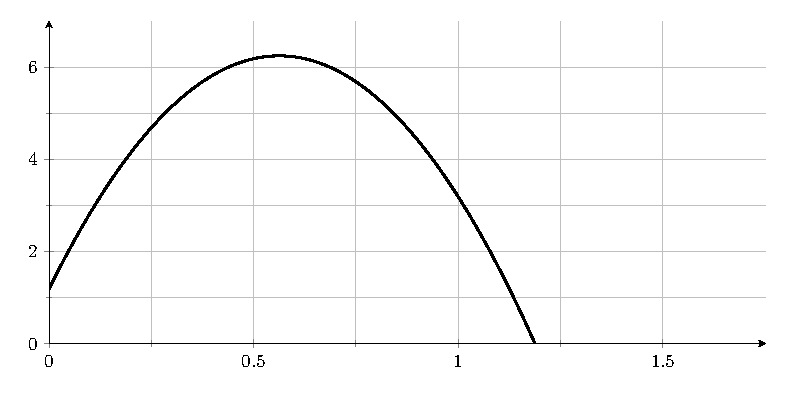
\includegraphics[width=.92\linewidth]{../figures/fhsm_2009_p32_1.pdf}
    \end{center}

    Các biểu thức (a)--(d) dưới đây là tương đương nhau. Biểu thức nào hữu ích nhất để tìm độ cao lớn nhất của móng ngựa, và vì sao đó là biểu thức hữu ích nhất?

    \begin{description}
      \item [\normalfont (a)] $1\frac{3}{16}+18t-16t^2$

      \item [\normalfont (b)] $-16\left(t-\frac{19}{16}\right)\left(t+\frac{1}{16}\right)$

      \item [\normalfont (c)] $\frac{1}{16}\left(19-16t\right)\left(16t+1\right)$

      \item [\normalfont (d)] $-16\left(t-\frac{9}{16}\right)^2+\frac{100}{16}$
    \end{description}

    \textbf{Trong lớp học (Đại số năm thứ hai)}

    \emph{Báo cáo nhóm:}

    \begin{quote}
      Chúng em loại biểu thức (a). Nó cho biết độ cao ban đầu và tốc độ đi lên ban đầu, nhưng câu hỏi không hỏi về điều nào trong hai điều đó. Các biểu thức (b) và (c) hầu như giống nhau, chỉ khác là ở (c), mẫu số trong các thừa số đã được đưa ra phía trước. Một bạn trong nhóm dùng (b) để tìm các nghiệm $\left(\frac{19}{16} \text{ và } -\frac{1}{16}\right)$, rồi tìm trung điểm $\left(\frac{9}{16}\right)$, đó phải là thời điểm đạt độ cao lớn nhất. Nhưng cuối cùng chúng em chọn (d), vì hạng tử
      $$
        -16\left(t-\frac{9}{16}\right)^2
      $$
      luôn âm hoặc bằng không, nên chúng em thấy rằng độ cao không bao giờ vượt quá $\frac{100}{16}$ foot, hay $6\frac{1}{4}$ foot, và đạt tới độ cao này tại $t=\frac{9}{16}$ giây, đúng bằng trung điểm tìm được khi dùng (b).
    \end{quote}

    \textbf{Các yếu tố then chốt của toán học}

    \begin{hanglist}
      \hangitem{Luận với kí hiệu đại số---Sử dụng kí hiệu có nghĩa; Liên kết biểu thức và hàm số}\vspace{\baselineskip}
    \end{hanglist}

    \textbf{Thói quen luận}
    
    \begin{hanglist}
      \hangitem{Phân tích bài toán---tìm kiếm cấu trúc ẩn}\vspace{\baselineskip}

      \hangitem{Phản tư về lời giải---diễn giải lời giải; biện minh hoặc kiểm chứng lời giải}
    \end{hanglist}
  }{}

\TriPara
  {
    \EN{Example 5 also raises a common difficulty to which teachers may need to be sensitive---confusion between a representation of the actual flight of an object (in this instance a horseshoe) and the time-versus-height graph. To help clarify this issue, teachers might ask such questions as ``How far do you think the horseshoe would travel?'' (certainly more than $1.2$ feet) or ``How do the scales of the two axes compare?''}
  }
  {
    \VI{Ví dụ 5 cũng làm nổi bật một khó khăn phổ biến mà giáo viên cần lưu ý---sự nhầm lẫn giữa hình biểu diễn đường bay thực tế của một vật (trong trường hợp này là chiếc móng ngựa) và đồ thị thời gian - độ cao. Để làm rõ vấn đề này, giáo viên có thể đặt những câu hỏi như: ``Theo em, chiếc móng ngựa sẽ bay được bao xa?'' (chắc chắn lớn hơn $1.2$ foot) hoặc ``Thang đo trên hai trục khác nhau như thế nào?''}
  }
  {
    \NOTE{
    Khó khăn được nhắc đến ở đây là sự lẫn lộn giữa hai loại hình biểu diễn rất khác nhau. Một hình biểu diễn đường bay thực tế của chiếc móng ngựa sẽ cho ta biết nó đang ở đâu trong không gian: theo phương ngang nó đã đi được bao xa, và theo phương thẳng đứng nó đang cao bao nhiêu. Nhưng đồ thị trong ví dụ này không biểu diễn vị trí không gian ấy. Đây là đồ thị thời gian--độ cao: trục ngang biểu thị thời gian tính từ lúc chiếc móng ngựa rời tay, còn trục dọc biểu thị độ cao của nó. Vì vậy, một điểm trên đồ thị không có nghĩa là chiếc móng ngựa đang ở vị trí đó trong mặt phẳng thật; điểm ấy chỉ nói rằng sau từng ấy giây, chiếc móng ngựa có độ cao từng ấy foot.

    Sự nhầm lẫn dễ xảy ra vì đường cong trên đồ thị cũng có dạng parabol. Trong kinh nghiệm học toán và vật lí, học sinh thường được biết rằng quỹ đạo của vật ném xiên, nếu bỏ qua sức cản không khí, có dạng parabol. Nhưng cần phân biệt hai parabol khác nhau. Nếu muốn biểu diễn quỹ đạo bay trong mặt phẳng thẳng đứng, trục ngang phải là khoảng cách ngang và trục dọc là độ cao; đó là đồ thị dạng $h=f(x)$. Còn trong ví dụ này, công thức đang cho là $h(t)=1\frac{3}{16}+18t-16t^2$, trong đó biến vào là thời gian $t$; đây là đồ thị dạng $h=f(t)$. Cùng là độ cao, nhưng một bên đặt độ cao trong quan hệ với khoảng cách ngang, một bên đặt độ cao trong quan hệ với thời gian. Vì vậy, tuy hai hình có thể đều là parabol, chúng không trả lời cùng một câu hỏi.

    Từ đó mới hiểu vì sao giáo viên có thể hỏi: ``Theo em, chiếc móng ngựa sẽ bay được bao xa?'' Câu hỏi này không nhằm yêu cầu học sinh tính ngay một con số chính xác, mà nhằm làm lộ ra việc các em có đang đọc nhầm trục ngang hay không. Khi đồ thị chạm trục ngang ở khoảng $t=1.2$, điều đó chỉ có nghĩa là chiếc móng ngựa chạm đất sau khoảng $1.2$ giây. Nó không có nghĩa là chiếc móng ngựa bay xa $1.2$ foot. Trên thực tế, khoảng cách bay theo phương ngang chắc chắn phải lớn hơn nhiều so với $1.2$ foot, nhưng đồ thị đang có không cho ta đủ thông tin để xác định khoảng cách ấy. Muốn biết chiếc móng ngựa bay xa bao nhiêu, cần thêm thông tin về chuyển động ngang, chẳng hạn vận tốc ngang hoặc hàm vị trí ngang theo thời gian.

    Từ đây có thể phát triển thành một bài toán mở rộng tự nhiên. Chẳng hạn, giả sử ta quay lại chuyển động của chiếc móng ngựa và, sau khi theo dõi hình chiếu của nó trên mặt đất, ước lượng được rằng trong mô hình lí tưởng vận tốc theo phương ngang gần như không đổi, khoảng $16$ foot mỗi giây. Giả thiết này phù hợp với mô hình ném xiên cơ bản: bỏ qua sức cản không khí, lực tác dụng theo phương ngang được xem như không đáng kể, nên chuyển động ngang là chuyển động đều. Gọi $x$ là khoảng cách ngang, tính bằng foot, từ vị trí ném đến hình chiếu của chiếc móng ngựa trên mặt đất. Khi đó $x=16t$, nên $t=\frac{x}{16}$. Thay vào công thức độ cao ban đầu, ta được
    $$
    h(x)=1\frac{3}{16}+18\cdot\frac{x}{16}-16\left(\frac{x}{16}\right)^2
    =\frac{19}{16}+\frac{9}{8}x-\frac{1}{16}x^2.
    $$

    Do đó, trong mô hình lí tưởng này, hàm số biểu diễn quỹ đạo bay của chiếc móng ngựa là
    $$
    h(x)=\frac{19}{16}+\frac{9}{8}x-\frac{1}{16}x^2
    =-\frac{1}{16}(x-19)(x+1).
    $$

    Nghiệm có ý nghĩa thực tế là $x=19$, nên chiếc móng ngựa bay xa khoảng $19$ foot trước khi chạm đất. Bài toán mở rộng này cho thấy rõ: để chuyển từ đồ thị $h(t)$ sang đồ thị quỹ đạo $h(x)$, không thể chỉ nhìn vào hình dạng parabol; phải có thêm thông tin về chuyển động ngang, chẳng hạn vận tốc ngang được đo hoặc ước lượng từ quan sát.

    Câu hỏi ``Thang đo trên hai trục khác nhau như thế nào?'' cũng nhằm kéo học sinh trở lại cách đọc đúng của đồ thị. Hai trục ở đây không cùng đại lượng và cũng không cùng đơn vị: trục ngang đo thời gian bằng giây, trục dọc đo độ cao bằng foot. Vì vậy, không thể nhìn hình như một bức tranh hình học của đường bay, cũng không thể so sánh trực tiếp một đoạn trên trục ngang với một đoạn trên trục dọc như thể cả hai đều là độ dài trong không gian. Giá trị sư phạm của ví dụ nằm ở chỗ nó buộc học sinh nhận ra rằng một đồ thị hàm số không tự nó là hình ảnh của hiện tượng; muốn hiểu đồ thị, trước hết phải đọc đúng mỗi trục biểu thị đại lượng nào, đơn vị nào, và quan hệ nào đang được mô hình hóa.
    }
  }

\ParallelSection
  {Mindful Manipulation}
  {Biến đổi có ý thức}
  {}

\TriPara
{
  \EN{Mindful manipulation includes learning algebraic manipulation as a process guided by understanding and goals (how do I want to use this expression, and what will make it most useful for this purpose?) and seeing that the basic rules of arithmetic provide a rationale for all legitimate manipulations of polynomial expressions. Of these, the distributive property, which is the only rule connecting the operations of addition and multiplication, is the one to which we must constantly appeal when doing anything that involves both operations at once, including a wide range of manipulations: expanding, factoring, collecting like terms, and putting fractions over a common denominator. Example 6 illustrates the difference between mindless and mindful manipulation when multiplying polynomials. It also illustrates the importance of organizing one's solution.}
}
{
  \VI{Biến đổi có ý thức bao gồm việc học biến đổi đại số như một quá trình được dẫn dắt bởi sự hiểu và mục tiêu (ta muốn sử dụng biểu thức này để làm gì, và điều gì sẽ khiến nó hữu ích nhất cho mục đích đó?), đồng thời nhận ra rằng quy tắc cơ bản của số học cung cấp cơ sở lí giải cho mọi phép biến đổi hợp lệ trên biểu thức đa thức. Trong số đó, tính chất phân phối, vốn là quy tắc duy nhất kết nối hai phép toán cộng và nhân, là quy tắc ta phải liên tục viện đến khi thực hiện bất kì thao tác nào liên quan đồng thời đến cả hai phép toán, bao gồm nhiều phép biến đổi: khai triển, phân tích thành nhân tử, thu gọn hạng tử đồng dạng, và quy đồng mẫu số. Ví dụ 6 minh họa sự khác biệt giữa biến đổi máy móc và biến đổi có ý thức khi nhân đa thức. Ví dụ này cũng cho thấy tầm quan trọng của việc tổ chức lời giải.}
}{\NOTE{}}

\TriExample
  {Distribute Thoroughly}
  {
    \textbf{Task}

    Expand:

    \begin{description}
      \item [\normalfont (a)] $(1 + x^3)(1 + x + x^2)$
      \item [\normalfont (b)] $(1 + x)(1 + x + x^2)$
    \end{description}\vspace{.25\baselineskip}

    \textbf{In the Classroom (First-Year Algebra)}

    Student 1 is accustomed to using the mnemonic FOIL (First, Outer, Inner, Last) to expand products of two binomials, such as $(1 + x)(1 + x^2)$, and applies it to the problem $(1 + x^3)(1 + x + x^2)$, getting $1 + x^2 + x^3 + x^5$.\vspace{\baselineskip}

    Student 2 says, ``You missed the products of the middle term, x, in the second factor. The distributive property means we have to multiply each term of one factor with each term of the other, and then add all the products.

    So I get
    $$
    \begin{aligned}
      &(1 + x^3)(1 + x + x^2) \\ 
        &\quad= 1 \cdot 1 + 1 \cdot x + 1 \cdot x^2 + x^3 \cdot 1\\
        &\qquad + x^3 \cdot x + x^3 \cdot x^2 \\
        &\quad= 1 + x + x^2 + x^3 + x^4 + x^5.
    \end{aligned}
    $$

    I sometimes remember this as `each with each.' Sometimes you can just multiply the terms mentally. I like to visualize the steps and write as little as possible. For example, when I apply `each with each' to\vspace{\baselineskip}

    $$
    \begin{aligned}
      &(1 - x)(1 + x + x^2) \\
      &\quad = 1 + x + x^2 - x - x^2 - x^3 \\
      &\quad = 1 - x^3,
    \end{aligned}
    $$
    I can see that the second and third terms from the multiplication by $1$ are opposites of the first and second terms from multiplication by $-x$, so I can just write down the remaining terms.''

    \textbf{Key Elements of Mathematics}

    \begin{hanglist}
      \hangitem{Reasoning with Algebraic Symbols---Meaningful use of symbols; Mindful manipulation}

      \hangitem{Reasoning with Numbers and Measurements---Number systems}
    \end{hanglist}


    \textbf{Reasoning Habits}

    \begin{hanglist}
      \hangitem{Analyzing a problem---applying previously learned concepts}

      \hangitem{Implementing a strategy---making purposeful use of procedures; organizing the solution}

      \hangitem{Seeking and using connections}
    \end{hanglist}
  }
  {Phân phối triệt để}
  {
    \textbf{Nhiệm vụ}

    Khai triển: 

    \begin{description}
      \item [\normalfont (a)] $(1 + x^3)(1 + x + x^2)$
      \item [\normalfont (b)] $(1 + x)(1 + x + x^2)$
    \end{description}

    \textbf{Trong lớp học (Đại số năm thứ nhất)}

    Học sinh 1 đã quen dùng mẹo nhớ FOIL (First, Outer, Inner, Last: hạng đầu, hạng ngoài, hạng trong, hạng cuối) để khai triển tích của hai nhị thức, chẳng hạn như $(1 + x)(1 + x^2)$, rồi áp dụng mẹo đó vào bài toán $(1 + x^3)(1 + x + x^2)$ và thu được $1 + x^2 + x^3 + x^5$.

    Học sinh 2 nói: ``Bạn đã bỏ sót các tích chứa hạng tử ở giữa, $x$, trong thừa số thứ hai. Tính chất phân phối có nghĩa là ta phải nhân mỗi hạng tử của một thừa số với mỗi hạng tử của thừa số kia, rồi cộng tất cả các tích.

    Vì thế mình được
    $$
    \begin{aligned}
      &(1 + x^3)(1 + x + x^2) \\
        &\quad= 1 \cdot 1 + 1 \cdot x + 1 \cdot x^2 + x^3 \cdot 1 \\
        &\qquad + x^3 \cdot x + x^3 \cdot x^2 \\
        &\quad= 1 + x + x^2 + x^3 + x^4 + x^5.
    \end{aligned}
    $$

    Đôi khi mình nhớ điều này bằng câu `mỗi hạng tử với mỗi hạng tử.' Đôi khi ta có thể nhân các hạng tử ngay trong đầu. Mình thích hình dung các bước và viết ít nhất có thể. Chẳng hạn, khi mình áp dụng `mỗi hạng tử với mỗi hạng tử' vào

    $$
    \begin{aligned}
      &(1 - x)(1 + x + x^2) \\
      &\quad = 1 + x + x^2 - x - x^2 - x^3 \\
      &\quad = 1 - x^3,
    \end{aligned}
    $$
    mình có thể thấy hạng tử thứ hai và thứ ba từ phép nhân với $1$ đối nhau với hạng tử thứ nhất và thứ hai từ phép nhân với $-x$, nên mình chỉ cần viết ra những hạng tử còn lại.''\vspace{\baselineskip}

    \textbf{Các yếu tố then chốt của toán học}

    \begin{hanglist}
      \hangitem{Luận với kí hiệu đại số---Sử dụng kí hiệu có nghĩa; Biến đổi có ý thức}\vspace{\baselineskip}

      \hangitem{Luận với số và đo lường---Hệ thống số}\vspace{\baselineskip}
    \end{hanglist}    

    \textbf{Thói quen luận}

    \begin{hanglist}
      \hangitem{Phân tích bài toán---vận dụng khái niệm đã học}

      \hangitem{Triển khai chiến lược---vận dụng thủ tục có chủ đích; tổ chức lời giải}\vspace{\baselineskip}

      \hangitem{Tìm kiếm và sử dụng kết nối}
    \end{hanglist}    
  }
  {
    \vspace{.5\baselineskip}
    FOIL chỉ áp dụng trực tiếp cho tích của hai nhị thức, tức là khi mỗi ngoặc đều chỉ có hai hạng tử. Chẳng hạn, với
    $$
    (1+x)(1+x^2),
    $$
    cả hai ngoặc đều là nhị thức, nên ta có thể lần lượt lấy hạng đầu, hạng ngoài, hạng trong và hạng cuối để được
    $$
    (1+x)(1+x^2)=1+x^2+x+x^3.
    $$

    Nhưng với
    $$
    (1+x^3)(1+x+x^2),
    $$
    ngoặc thứ hai có ba hạng tử, nên không còn là nhị thức nữa. Vì vậy, FOIL không còn thích hợp. Nếu vẫn áp dụng máy móc, học sinh sẽ chỉ lấy bốn tích như $1\cdot1=1$, $1\cdot x^2=x^2$, $x^3\cdot1=x^3$, $x^3\cdot x^2=x^5$, mà bỏ sót hai tích $1\cdot x=x$ và $x^3\cdot x=x^4$. Bởi thế, kết quả
    $$
    1+x^2+x^3+x^5
    $$
    là chưa đầy đủ.

    Khai triển đúng phải là
    $$
    (1+x^3)(1+x+x^2)=1+x+x^2+x^3+x^4+x^5.
    $$

    Điểm đáng chú ý ở đây là học sinh đã dùng một mẹo quen thuộc trong một tình huống mà nó không còn phù hợp. Vì vậy, ví dụ này làm lộ ra một hạn chế quan trọng của việc học theo thủ tục: học sinh có thể nhớ cách làm, nhưng chưa thật sự hiểu vì sao thủ tục ấy đúng và khi nào thì có thể dùng nó.
  }

\ParallelSection
  {Reasoned Solving}
  {Giải có cơ sở luận}
  {}

\TriPara
  {
    \EN{Equation solving is a goal-oriented process of logical argument; it is based on general principles of equality and procedures of algebraic manipulation consistent with the rules of arithmetic. Problem solving with equations should include careful attention to increasingly difficult problems that span the border between arithmetic and algebra. Such problems can help students view algebra as a sense-making activity that extends one's problem-solving skills into domains in which reasoning as done in arithmetic becomes too complicated or cumbersome to carry out. Seeing the essential parallels between algebraic and arithmetic solution methods can help students realize that algebra is not something totally new but simply a more powerful tool for dealing with problems that are hard to approach with arithmetic by itself (Saul 2001). In example 7 we illustrate reasoned solving of equations. Worth noting is the fact that although one student used a standard algebraic approach and the other used reasoning based on the concrete context, the steps in their solutions are essentially the same. Examples of this sort can help students see algebra as an extension of concrete arithmetic reasoning.}
  }
  {
    \VI{Giải phương trình là một quá trình lập luận logic có định hướng mục tiêu; quá trình ấy dựa trên những nguyên lí chung về đẳng thức và các thủ tục biến đổi đại số phù hợp với quy tắc số học. Giải quyết vấn đề bằng phương trình cần chú ý cẩn trọng đến những bài toán ngày càng khó hơn, nằm ở vùng ranh giới giữa số học và đại số. Những bài toán như vậy có thể giúp học sinh nhìn đại số như một hoạt động hiểu, mở rộng kĩ năng giải quyết vấn đề sang những miền mà cách luận theo số học trở nên quá phức tạp hoặc quá cồng kềnh để thực hiện. Việc nhìn ra những tương đồng cốt yếu giữa phương pháp giải đại số và phương pháp giải số học có thể giúp học sinh nhận ra rằng đại số không phải là điều hoàn toàn mới, mà chỉ là một công cụ mạnh hơn để xử lí những bài toán khó tiếp cận nếu chỉ dùng riêng số học (Saul 2001). Trong Ví dụ 7, chúng tôi minh họa việc giải phương trình có cơ sở luận. Điều đáng lưu ý là mặc dù một học sinh dùng cách tiếp cận đại số chuẩn, còn học sinh kia dùng lối luận dựa trên ngữ cảnh cụ thể, các bước trong hai lời giải về thực chất là như nhau. Những ví dụ kiểu này có thể giúp học sinh nhìn đại số như sự mở rộng của luận số học cụ thể.}
  }
  {
    \NOTE{
    Đoạn này cho thấy hiểu không phải là một bước phụ sau khi đã học xong thủ tục đại số, mà là điều kiện để đại số trở thành một hoạt động toán học có nghĩa. Nếu học sinh chỉ học giải phương trình như một chuỗi thao tác biến đổi kí hiệu, các em có thể làm được một số bài quen thuộc nhưng khó thấy vì sao các thao tác ấy hợp lí, và càng khó biết khi nào nên dùng đại số để giải quyết một tình huống mới. Ngược lại, khi học sinh nhận ra rằng lời giải đại số có những tương đồng cốt yếu với cách luận số học đã quen thuộc, đại số bắt đầu trở nên rõ nghĩa: nó không còn là một hệ kí hiệu xa lạ, mà là sự mở rộng mạnh hơn của những cách nghĩ đã có.

    Theo nghĩa này, hiểu là một đặc trưng không thể thiếu của hoạt động toán học thực chất. Làm toán không chỉ là thực hiện thủ tục đúng, mà còn là liên tục diễn giải tình huống, nhận ra cấu trúc, chọn biểu diễn thích hợp, kết nối cái mới với cái đã biết, và kiểm tra xem lời giải có thật sự trả lời vấn đề đang đặt ra hay không. Chính quá trình ấy giúp người học chuyển từ số học sang đại số một cách tự nhiên: từ xử lí các con số cụ thể sang xử lí quan hệ bằng kí hiệu. Vì vậy, đại số không thay thế luận số học, mà khái quát hóa và làm cho nó trở nên linh hoạt hơn trong những bài toán mà cách làm số học riêng lẻ trở nên quá cồng kềnh.
}
  }

\TriExample
  {Finding Balance}
  {
    \textbf{Task}

    A slab of soap on one pan of a scale balances $\frac{3}{4}$ of a slab of soap of equal weight and a $\frac{3}{4}$-pound weight on the other pan. How much does the slab of soap weigh? Solve the problem both with an algebraic equation and by direct arithmetic reasoning.  (Adapted from Kordemsky and Parry [1992])

    \textbf{In the Classroom (Ninth-Grade Students' Solutions)}

    \begin{scriptlist}
      \item [Student 1:] If $x$ is the weight of the slab in pounds, then one side of the balance weighs $x$ pounds and the other weighs
      $$
      \frac{3}{4}x+\frac{3}{4},
      $$
      so
      $$
      x=\frac{3}{4}x+\frac{3}{4}.
      $$

      Subtracting $\frac{3}{4}x$ from both sides gives
      $$
      \frac{1}{4}x=\frac{3}{4}
      $$
      so $x=3$.\vspace{.5\baselineskip}

      \item [Student 2:] It's just as easy without equations! If a slab of soap balances $\frac{3}{4}$ of a slab and $\frac{3}{4}$ pound, take $\frac{3}{4}$ of a slab off each side. That leaves $\frac{1}{4}$ of a slab on one side and $\frac{3}{4}$ pound on the other. So a quarter of a slab weighs $\frac{3}{4}$ of a pound. A full slab is four quarters, and that will make $3$ pounds.\vspace{2\baselineskip}
      
      \item [Teacher:] Good! Can you see the connection between your two solutions?
      
      \item [Student 1:] Oh, I see. What she did is really the same except she didn't use an $x$.
    \end{scriptlist}

    \textbf{Key Mathematical Elements}

    \begin{hanglist}
      \hangitem{Reasoning with Algebraic Symbols---Meaningful use of symbols; Reasoned solving}
    \end{hanglist}    

    \textbf{Reasoning Habits}

    \begin{hanglist}
      \hangitem{Implementing a strategy---making purposeful use of procedures; making logical deductions}

      \hangitem{Seeking and using connections}
    \end{hanglist}    
  }
  {
    Tìm thế cân bằng
  }
  {
    \textbf{Nhiệm vụ}

    Một bánh xà phòng đặt trên một đĩa cân thì cân bằng với $\frac{3}{4}$ bánh xà phòng có cùng khối lượng và một quả cân $\frac{3}{4}$ pound\footnote{Pound (lb): đơn vị đo khối lượng trong hệ Mĩ; $1\;\text{lb}=.45\;\text{kg}$.} đặt trên đĩa bên kia. Bánh xà phòng nặng bao nhiêu? Hãy giải bài toán bằng cả phương trình đại số lẫn luận số học trực tiếp. (Phỏng theo Kordemsky and Parry [1992])

    \textbf{Trong lớp học (Lời giải của học sinh lớp 9\footnote{Trong bản dịch này, ``lớp 9'' dùng để chuyển \emph{ninth grade} trong hệ giáo dục Hoa Kì. Đây thường là năm đầu của bậc \emph{high school} trong mô hình phổ biến gồm Grade 9--12, dù cách tổ chức cụ thể có thể khác nhau theo bang hoặc học khu; vì vậy không nên hiểu máy móc là lớp 9 thuộc bậc trung học cơ sở như trong hệ giáo dục Việt Nam hiện nay.})}

    \begin{scriptlist}
    \item [Học sinh 1:] Nếu gọi $x$ là khối lượng của bánh xà phòng, tính theo pound, thì một bên cân nặng $x$ pound, còn bên kia nặng
    $$
    \frac{3}{4}x+\frac{3}{4},
    $$
    nên
    $$
    x=\frac{3}{4}x+\frac{3}{4}.
    $$

    Trừ $\frac{3}{4}x$ ở cả hai vế, ta được
    $$
    \frac{1}{4}x=\frac{3}{4}
    $$
    nên $x=3$.

    \item [Học sinh 2:] Không dùng phương trình thì bài này cũng dễ như vậy thôi! Nếu một bánh xà phòng cân bằng với $\frac{3}{4}$ bánh xà phòng và $\frac{3}{4}$ pound, thì lấy $\frac{3}{4}$ bánh xà phòng ra khỏi mỗi bên. Khi đó còn lại $\frac{1}{4}$ bánh xà phòng ở một bên và $\frac{3}{4}$ pound ở bên kia. Vậy một phần tư bánh xà phòng nặng $\frac{3}{4}$ pound. Một bánh đầy đủ gồm bốn phần tư, nên sẽ nặng $3$ pound.
    
    \item [Giáo viên:] Tốt! Các em có nhìn ra mối liên hệ giữa hai lời giải của mình không?
    
    \item [Học sinh 1:] À, em hiểu rồi. Cách bạn ấy làm thực ra cũng giống hệt, chỉ là bạn ấy không dùng $x$.
    \end{scriptlist}

    \noindent\textbf{Các yếu tố then chốt của toán học}

    \begin{hanglist}
      \hangitem{Luận với kí hiệu đại số---Sử dụng kí hiệu có nghĩa; Giải có cơ sở luận}\vspace{\baselineskip}
    \end{hanglist}

    \noindent\textbf{Thói quen luận}

    \begin{hanglist}
      \hangitem{Triển khai chiến lược---vận dụng thủ tục có chủ đích; thực hiện suy diễn logic}\vspace{\baselineskip}

      \hangitem{Tìm kiếm và sử dụng kết nối}
    \end{hanglist}
  }{}

\ParallelSection
  {Connecting Algebra with Geometry}
  {Kết nối đại số với hình học}
  {}

\TriPara
  {
    \EN{An interplay exists between algebra and geometry: such geometric representations as graphs or figures can cast light on algebraic expressions and equations, and algebraic representations can be used to deduce geometric relationships (Katz 2007). Example 8 shows how the area model given in example 4, ``A Model Idea,'' can be extended in a geometrically compelling way to help students make sense of completing the square, a process that students often find mysterious. This example additionally illustrates the power of an effective representation as a basis for reasoning and shows how structure can be uncovered in that representation to move toward a general solution.}
  }
  {
    \VI{Giữa đại số và hình học có sự tác động qua lại: những biểu diễn hình học như đồ thị hoặc hình vẽ có thể làm sáng tỏ biểu thức và phương trình đại số, còn biểu diễn đại số có thể được dùng để suy ra quan hệ hình học (Katz 2007). Ví dụ 8 cho thấy cách mô hình diện tích được nêu trong Ví dụ 4, ``Những mảnh ghép đại số'', có thể được mở rộng theo một cách thuyết phục về hình học để giúp học sinh hiểu quá trình hoàn thành bình phương, vốn là một quá trình học sinh thường thấy khó nắm bắt. Ví dụ này đồng thời minh họa sức mạnh của một biểu diễn hiệu quả như cơ sở cho luận, và cho thấy cách cấu trúc có thể được phát hiện trong chính biểu diễn ấy để hướng tới lời giải tổng quát.}
  }{\NOTE{}}

\TriExample
  {Squaring It Away}
  {
    \textbf{Task}

    Find a way of solving the equation $x^2 + 10x = 144$ by using an area model.

    \textbf{In the Classroom (Intermediate Algebra Class)}

    \begin{scriptlist}
      \item [Teacher:] Can anybody see how to think of $x^2 + 10x$ as an area?\vspace{\baselineskip}
      
      \item [Student 1:] Well, $x^2$ is the area of a square with side $x$, and $10x$ is the area of a rectangle with sides $x$ and $10$, so we can put the rectangle and the square together like this. [See the figure at the right.] But I don't see how this helps.\vspace{\baselineskip}
      
      \begin{center}
      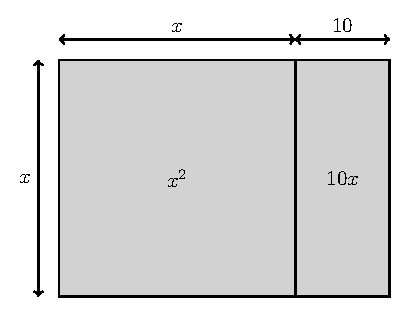
\includegraphics[width=.92\linewidth]{../figures/fhsm_2009_p36_1.pdf}
      \end{center}

      \item [Student 2:] Maybe if we knew what the area of the square was, we could just take the square root to find $x$.
      
      \item [Teacher:] Is there a way of rearranging the figure so that it's close to being a square?
      
      \item [Student 1:] I know! If we cut the rectangle into two rectangles of width $5$, we could put one on each side like this! [See the figure at the right.]
      
      \begin{center}
      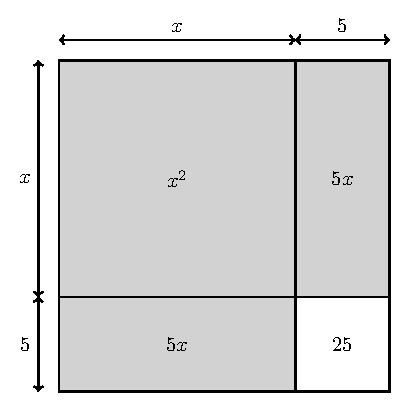
\includegraphics[width=.92\linewidth]{../figures/fhsm_2009_p36_2.pdf}
      \end{center}

      \item [Student 2:] But it's not a complete square, it's missing a corner.\vspace{\baselineskip}
      
      \item [Teacher:] What's the area of the corner?\vspace{\baselineskip}
      
      \item [Student 2:] Oh, it must be $25$, since the white square lines up with ends of the rectangles, so it has side length $5$. And since the gray area is $144$, the entire area of the big square is $144 + 25 = 169$.
      
      \item [Student 1:] And that means the side length of the square is $13$, so $x + 5 = 13$, which means $x = 8$.
      
      \item [Student 2:] Shouldn't there be another solution, since the $(x + 5)$ is squared?
      
      \item [Teacher:] Interesting point. Let's take a closer look. Can you write down what you did algebraically?
      
      \item [Student 2:] We started with $x^2 + 10x = 144$, and then we added $25$ to the $144$. I guess that means we add $25$ to both sides of the equation, so we get $x^2 + 10x + 25 = 169$.\vspace{\baselineskip}
      
      \item [Student 1:] So to get $25$, we divide the $10$ by $2$ to get $5$, then square that to get $25$.
      
      \item [Student 2:] Yeah, and then the left-hand side is a perfect square, so you get $(x + 5)^2 = 169$.
      
      \item [Student 1:] The algebraic way gives you both solutions, because you get $x + 5 = 13$ or $x + 5 = -13$, so $x = 8$ or $x = -18$, but I guess the area model can't give you the negative solution.
      
      \item [Teacher:] Good observations. The process of adding a constant to a quadratic expression so that it becomes a perfect square is called ``completing the square.'' In the geometric interpretation, you just found that constant by adding in a corner piece. Can you see how this process might work for other quadratic equations?
    \end{scriptlist}\vspace{\baselineskip}

    The teacher could continue this discussion to lead to the development of the quadratic formula.

    \textbf{Key Mathematical Elements}

    \begin{hanglist}
      \hangitem{Reasoning with Algebraic Symbols---Meaningful use of symbols; Mindful manipulation; Connecting algebra with geometry}
    \end{hanglist}

    \textbf{Reasoning Habits}

    \begin{hanglist}
      \hangitem{Analyzing a problem---looking for hidden structure}

      \hangitem{Seeking and using connections}

      \hangitem{Reflecting on a solution---revisiting initial assumptions; generalizing a solution}
    \end{hanglist}    
  }
  {Ổn thỏa bình phương}
  {
    \textbf{Nhiệm vụ}

    Tìm một cách giải phương trình $x^2 + 10x = 144$ bằng mô hình diện tích.

    \textbf{Trong lớp học (Đại số trung cấp)}\vspace{\baselineskip}

    \begin{scriptlist}
    \item [Giáo viên:] Có bạn nào thấy có thể nghĩ về $x^2 + 10x$ như một diện tích không?
    
    \item [Học sinh 1:] Dạ, $x^2$ là diện tích hình vuông cạnh $x$, còn $10x$ là diện tích hình chữ nhật có hai cạnh $x$ và $10$, nên ta có thể ghép hình chữ nhật và hình vuông với nhau như thế này. [Xem hình bên dưới.] Nhưng em chưa thấy điều này giúp ích thế nào.\vspace{\baselineskip}
    
    \begin{center}
        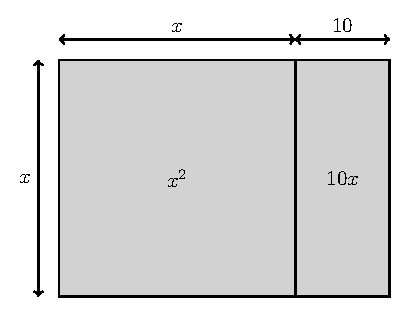
\includegraphics[width=.92\linewidth]{../figures/fhsm_2009_p36_1.pdf}
    \end{center}

    \item [Học sinh 2:] Có lẽ nếu biết diện tích hình vuông là bao nhiêu thì ta chỉ việc lấy căn bậc hai để tìm $x$.\vspace{\baselineskip}
    
    \item [Giáo viên:] Có cách nào sắp xếp lại hình để nó gần thành hình vuông không?
    
    \item [Học sinh 1:] Em biết rồi! Nếu cắt hình chữ nhật thành hai hình chữ nhật có chiều rộng $5$, ta có thể đặt mỗi hình vào một bên như thế này! [Xem hình bên dưới.]
    
    \begin{center}
        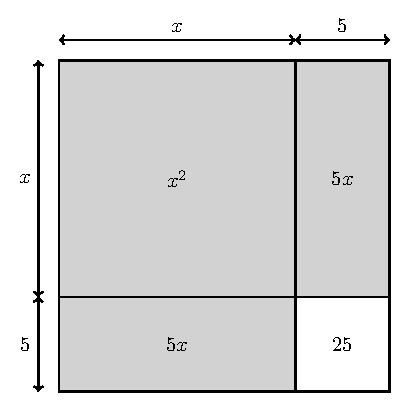
\includegraphics[width=.92\linewidth]{../figures/fhsm_2009_p36_2.pdf}
    \end{center}

    \item [Học sinh 2:] Nhưng nó chưa phải là hình vuông hoàn chỉnh, nó còn thiếu một góc.
    
    \item [Giáo viên:] Diện tích của phần góc ấy là bao nhiêu?
    
    \item [Học sinh 2:] À, chắc phải là $25$, vì hình vuông trắng thẳng hàng với đầu của các hình chữ nhật, nên nó có cạnh dài $5$. Và vì phần màu xám có diện tích $144$, nên toàn bộ diện tích hình vuông lớn là $144 + 25 = 169$.
    
    \item [Học sinh 1:] Và điều đó có nghĩa là cạnh của hình vuông là $13$, nên $x + 5 = 13$, suy ra $x = 8$.
    
    \item [Học sinh 2:] Chẳng phải phải có thêm một nghiệm nữa sao, vì $(x + 5)$ được bình phương?
    
    \item [Giáo viên:] Nhận xét thú vị đấy. Ta hãy xem kĩ hơn. Em có thể viết lại bằng đại số điều em vừa làm không?
    
    \item [Học sinh 2:] Chúng em bắt đầu với $x^2 + 10x = 144$, rồi cộng $25$ vào $144$. Chắc điều đó có nghĩa là phải cộng $25$ vào cả hai vế của phương trình, nên ta được $x^2 + 10x + 25 = 169$.
    
    \item [Học sinh 1:] Vậy để được $25$, ta lấy $10$ chia cho $2$ được $5$, rồi bình phương lên được $25$.
    
    \item [Học sinh 2:] Đúng, và khi đó vế trái là một bình phương hoàn chỉnh, nên ta được $(x + 5)^2 = 169$.
    
    \item [Học sinh 1:] Cách làm bằng đại số cho cả hai nghiệm, vì ta có $x + 5 = 13$ hoặc $x + 5 = -13$, nên $x = 8$ hoặc $x = -18$, nhưng em đoán mô hình diện tích không cho được nghiệm âm.
    
    \item [Giáo viên:] Những quan sát rất tốt. Quá trình cộng hằng số vào biểu thức bậc hai để nó trở thành một bình phương hoàn chỉnh được gọi là ``hoàn thành bình phương.'' Trong diễn giải hình học, các em vừa tìm ra hằng số ấy bằng cách thêm vào mảnh góc. Các em có thấy quá trình này có thể hoạt động như thế nào với những phương trình bậc hai khác không?
    \end{scriptlist}

    Giáo viên có thể tiếp tục cuộc thảo luận này để dẫn tới việc hình thành công thức nghiệm của phương trình bậc hai.

    \textbf{Các yếu tố then chốt của toán học}

    \begin{hanglist}
      \hangitem{Luận với kí hiệu đại số---Sử dụng kí hiệu có nghĩa; Biến đổi có ý thức; Kết nối đại số với hình học}\vspace{\baselineskip}
    \end{hanglist}    

    \textbf{Thói quen luận}

    \begin{hanglist}
      \hangitem{Phân tích bài toán---tìm kiếm cấu trúc ẩn}\vspace{\baselineskip}

      \hangitem{Tìm kiếm và sử dụng kết nối}

      \hangitem{Phản tư về lời giải---xem lại giả định ban đầu; khái quát hóa lời giải}
    \end{hanglist}
  }
  {
    \vspace{.5\baselineskip}
    Ví dụ 8 đáng chú ý ở chỗ nó cho thấy phép hoàn thành bình phương có thể được giảng dạy theo hướng nhắm tới \emph{cấu trúc đích}---bình phương bằng hằng số---thay vì thủ thuật cần ghi nhớ.

    Bình phương bằng hằng số là dạng quen thuộc và dễ xử lí, vì khi đó có thể giải bằng cách khai căn rồi xét các khả năng tương ứng. Từ điểm tựa ấy, phương trình
    $$
    x^2+10x=144
    $$
    không còn được đọc như biểu thức cần biến đổi máy móc, mà như biểu thức \emph{chưa đạt tới} cấu trúc mong muốn.

    Theo hướng đó, hằng số $25$ không xuất hiện như một mẹo, mà như phần tất yếu phải có để vế trái trở thành bình phương hoàn chỉnh, tức là
    $$
    x^2+10x+25=(x+5)^2.
    $$

    Vai trò của mô hình diện tích là làm lộ ra và biện minh cho sự xuất hiện của phần bù ấy. Nó giúp học sinh \emph{thấy vì sao} cần thêm mảnh góc có diện tích $25$, chứ không thay thế cho luận đại số. Chính ở điểm này, ví dụ cho thấy một biểu diễn hình học hiệu quả có thể nâng đỡ hiểu mà không làm mất đi bản chất của việc giải có cơ sở luận.

    Vì vậy, giá trị sư phạm của ví dụ không nằm riêng ở việc tìm ra nghiệm, mà ở chỗ nó làm sáng tỏ quan hệ giữa ba tầng: cấu trúc đại số cần đạt tới, biểu diễn hình học giúp soi sáng cấu trúc ấy, và thủ tục biến đổi hướng tới cấu trúc đó. Bởi thế, thuật ngữ \emph{hoàn thành bình phương} nên đến sau khi ý nghĩa của thao tác đã được dựng lên đủ rõ.

    Nếu dùng ví dụ này như một điểm tựa cấu trúc trong dạy học, thì mô hình diện tích cần được đặt đúng vai trò của nó: một phương tiện soi sáng và biện minh, chứ không phải con đường bắt buộc duy nhất. Cách tổ chức ấy vừa giữ được chiều trực quan cho những học sinh cần đến biểu diễn, vừa không che khuất lối đi của những học sinh đã có thể tiến thẳng bằng tư duy cấu trúc.
  }

\ParallelSection
  {Linking Expressions and Functions}
  {Liên kết biểu thức và hàm số}
  {}

\TriPara
  {
    \EN{Although multiple representations of functions---symbolic, graphical, numerical, and verbal---are commonly seen, the idea of multiple algebraic representations of functions is less commonly made explicit. Different but equivalent ways of writing the same function may reveal different properties of the function, as illustrated in example 5, ``Horseshoes in Flight.''}
  }
  {
    \VI{Mặc dù nhiều biểu diễn của hàm số---bằng kí hiệu, bằng đồ thị, bằng số và bằng lời---thường được nhắc đến, ý tưởng về nhiều biểu diễn đại số của hàm số lại ít khi được nêu rõ. Những cách viết khác nhau nhưng tương đương cho cùng một hàm số có thể làm lộ ra những tính chất khác nhau của hàm số, như đã minh họa trong Ví dụ 5, ``Móng ngựa trên không''.}
  }{\NOTE{}}

\TriPara
  {
    \EN{Symbolic representation shifts to a higher level when we start to use letters to stand for functions and introduce function notation (Saul 2001). The magnitude of this shift is often overlooked. High school students have difficulty with extending the four basic arithmetic operations to functions and also with composition of functions. Embedding these experiences in a context may enhance students' comprehension of the concepts and improve both their retention and their ability to make connections (Katz 2007), as in example 5, ``Horseshoes in Flight.'' Example 9 illustrates the power of using technology to link functions and expressions in an abstract mathematical context.}
  }
  {
    \VI{Biểu diễn kí hiệu chuyển sang cấp độ cao hơn khi ta bắt đầu dùng chữ cái để biểu thị hàm số và giới thiệu kí hiệu hàm (Saul 2001). Tầm vóc của sự chuyển dịch này thường bị xem nhẹ. Học sinh trung học phổ thông gặp khó khăn khi mở rộng bốn phép toán số học cơ bản sang hàm số, cũng như khi làm việc với phép hợp hàm. Việc đặt những trải nghiệm ấy vào ngữ cảnh cụ thể có thể giúp học sinh hiểu khái niệm tốt hơn, đồng thời cải thiện khả năng ghi nhớ và khả năng thiết lập kết nối (Katz 2007), như trong Ví dụ 5, ``Móng ngựa trên không''. Ví dụ 9 minh họa sức mạnh của việc dùng công nghệ để liên kết hàm số và biểu thức trong ngữ cảnh toán học trừu tượng.}
  }
  {
    \NOTE{Bước ngoặt quan trọng trong việc sử dụng kí hiệu là: chữ cái không còn chỉ đại diện cho số, mà còn có thể đại diện cho hàm số. Khi đó, học sinh không chỉ thao tác với các giá trị riêng lẻ, mà còn thao tác với chính các quan hệ phụ thuộc. Vì vậy, khó khăn với các biểu thức như $(f+g)(x)$, $(fg)(x)$ hay $f(g(x))$ không chỉ là khó khăn tính toán, mà còn là khó khăn trong việc hiểu đối tượng đang được xét và ý nghĩa của kí hiệu.

    Chính ở điểm này, việc đặt các kí hiệu và phép toán ấy vào ngữ cảnh cụ thể có giá trị sư phạm rõ rệt: nó giúp học sinh thấy các phép toán trên hàm số và phép hợp hàm không phải những biến đổi hình thức rời rạc, mà gắn với những quan hệ có nghĩa. Còn trong bối cảnh trừu tượng hơn, công nghệ có thể giúp liên kết biểu thức với sự vận hành của hàm số, nhờ đó làm sáng rõ các kết nối mà học sinh dễ bỏ sót nếu chỉ nhìn vào kí hiệu.}
  }

\TriPara
  {
    \EN{Building fluency in working with algebraic notation that is grounded in reasoning and sense making will ensure that students can flexibly apply the powerful tools of algebra in a variety of contexts both within and outside mathematics.}
  }
  {
    \VI{Việc xây dựng sự thành thạo trong khi làm việc với kí hiệu đại số, đặt nền trên luận và hiểu, sẽ bảo đảm rằng học sinh có thể vận dụng linh hoạt công cụ mạnh mẽ của đại số trong nhiều ngữ cảnh, cả trong lẫn ngoài toán học.}
  }{\NOTE{}}

\TriExampleLong
  {More Than Meets the Eye}
  {
    \textbf{Task}

    In earlier grades you may have seen problems that asked you to find the next term in a sequence, such as $3$, $7$, $11$. One possible answer is $15$, assuming the sequence is generated by evaluating $f(x) = 4x - 1$ at $x = 1, 2, 3$. But are other answers possible?
  }
  {
    Chưa thấy hết quy luật
  }
  {
    \textbf{Nhiệm vụ}

    Ở các lớp dưới, có thể các em đã từng gặp bài toán yêu cầu tìm số hạng tiếp theo của một dãy, chẳng hạn $3$, $7$, $11$. Câu trả lời có khả năng là $15$, nếu giả sử dãy được tạo ra bằng cách lấy giá trị của $f(x)=4x-1$ tại $x=1,2,3$. Nhưng có thể có câu trả lời khác không?
  }{}

\TriExampleLongNext
  {
    \textbf{In the Classroom (Fourth-Year Mathematics)}

    \begin{scriptlist}
      \item [Teacher:] Find the sequence generated by evaluating $g(x) = x^3 - 6x^2 + 15x - 7$ at $x = 1, 2, 3$.
      
      \item [Student:] I get $g(1) = 3$, $g(2) = 7$, and $g(3) = 11$. It's the same sequence: $3$, $7$, $11$.
      
      \item [Teacher:] What would be the next term if you used $g(x)$ instead of $f(x)$?
      
      \item [Student:] It would be $g(4) = 21$. That's different from what we get by using $f(x)$.
      
      \item [Teacher:] Can you find other polynomials that generate the sequence $3$, $7$, $11$?
      
      \item [Student:] I don't see how you came up with that weird cubic for $g$ in the first place.
      
      \item [Teacher:] What does it mean when we say that $g(1) = 3$?
      \item [Student:] Well, it means that the $y$-value, or output, is $3$ when the $x$-value, or input, is $1$.
      
      \item [Teacher:] So how can two different functions, $f$ and $g$, have the same values at $x = 1, 2, \text{ and } 3$?
      
      \item [Student:] I suppose that both of their graphs would have to have the same $y$-values.... Hey, that means they must intersect at those three points! Let me check that by graphing them. Yes, when I graph them, I see that the straight line graph of $f(x)$ intersects the cubic graph of $g(x)$ at $x = 1, 2, \text{ and } 3$.
        \begin{center}
          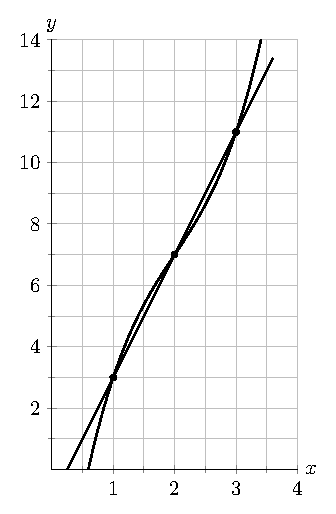
\includegraphics[width=.92\linewidth]{../figures/fhsm_2009_p38_1.pdf}
        \end{center}
    \end{scriptlist}
  }
  {
    \textbf{Trong lớp học (Toán năm thứ tư\footnote{\emph{Fourth-Year Mathematics} chỉ khóa toán năm thứ tư trong chuỗi môn toán bậc \emph{high school} ở hệ giáo dục Hoa Kì, thường tương ứng với năm cuối trong mô hình Grade 9--12. Cụm này không nên hiểu là ``toán lớp 4'' và cũng không mặc định là một khóa đại số; nội dung cụ thể có thể thay đổi theo bang, học khu hoặc chương trình học.})}\vspace{\baselineskip}

    \begin{scriptlist}
    \item [Giáo viên:] Hãy tìm dãy được sinh ra bằng cách tính giá trị của $g(x)=x^3-6x^2+15x-7$ tại $x=1,2,3$.

    \item [Học sinh:] Em được $g(1)=3$, $g(2)=7$, và $g(3)=11$. Vẫn là cùng dãy ấy: $3$, $7$, $11$.

    \item [Giáo viên:] Nếu dùng $g(x)$ thay cho $f(x)$ thì số hạng tiếp theo sẽ là gì?

    \item [Học sinh:] Khi đó sẽ là $g(4)=21$. Kết quả này khác với kết quả nhận được khi dùng $f(x)$.

    \item [Giáo viên:] Em có thể tìm những đa thức khác cũng sinh ra dãy $3$, $7$, $11$ không?

    \item [Học sinh:] Em không hiểu ngay từ đầu thầy nghĩ ra đa thức bậc ba lạ như vậy cho $g$ bằng cách nào.

    \item [Giáo viên:] Khi ta nói $g(1)=3$ thì điều đó có nghĩa là gì?

    \item [Học sinh:] Nghĩa là giá trị $y$, hay đầu ra, bằng $3$ khi giá trị $x$, hay đầu vào, bằng $1$.

    \item [Giáo viên:] Vậy làm sao hai hàm khác nhau, $f$ và $g$, lại có cùng giá trị tại $x=1,2,\text{ và }3$?
    
    \item [Học sinh:] Em đoán là đồ thị của cả hai hàm phải có cùng các giá trị $y$.... À, nghĩa là chúng phải cắt nhau tại ba điểm đó! Để em kiểm tra bằng cách vẽ đồ thị. Đúng rồi, khi vẽ đồ thị, em thấy đồ thị đường thẳng của $f(x)$ cắt đồ thị bậc ba của $g(x)$ tại $x=1,2,\text{ và }3$.
    
      \begin{center}
      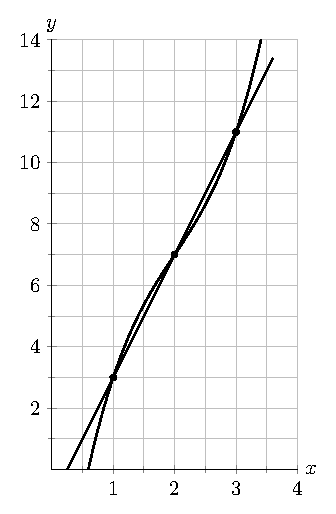
\includegraphics[width=.92\linewidth]{../figures/fhsm_2009_p38_1.pdf}
      \end{center}
    \end{scriptlist}
  }{}

\TriExampleLongNext
  {
    \begin{scriptlist}
      \item [Teacher:] Can you see now how you might find another polynomial graphically?
      
      \item [Student:] Maybe I could figure out a way to change the shape of the cubic graph but keep the intersection points the same.
      
      \item [Teacher:] How would you do that algebraically?
      
      \item [Student:] I could try to stretch the difference between $f(x)$ and $g(x)$, which is 
      $$
        g(x) - f(x) = x^3 - 6x^2 + 11x - 6.
      $$
      I could triple that, for example, and add it back on to $f(x)$ and get 
      $$
        \begin{aligned}
          &4x - 1 + 3(x^3 - 6x^2 + 11x - 6) \\
          &\quad= 3x^3 - 18x^2 + 37x - 19.
        \end{aligned}
      $$

      \item [Teacher:] Excellent. Now I want to understand what is really going on here. Is there anything special about the polynomial $x^3 - 6x^2 + 11x - 6$ that makes this work?
      
      \item [Student:] Not that I can see.
      
      \item [Teacher:] Why don't you try factoring it on your CAS?
    \end{scriptlist}

    \begin{center}
      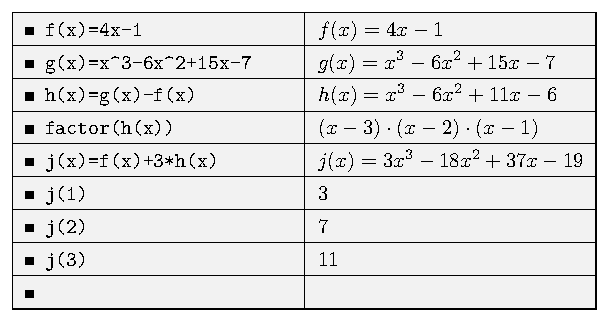
\includegraphics[width=.92\linewidth]{../figures/fhsm_2009_p39_f1.pdf}
    \end{center}

    \begin{scriptlist}  
      \item [Student:] I get   
      $$
        \begin{aligned}
          &x^3 - 6x^2 + 11x - 6 \\
          &\quad = (x - 1)(x - 2)(x - 3).
        \end{aligned}
      $$
      Oh, I see. When I look at the factored form, I can see that the difference between $f(x)$ and $g(x)$ is $0$ at $x = 1, 2, \text{ and } 3$. So I could get many polynomials that generate the same sequence just by adding a multiple of this polynomial to $f(x)$.

      \item [Teacher:] What is the general form of such a polynomial?
      
      \item [Student:] It is 
      $$
        4x - 1 + k(x - 1)(x - 2)(x - 3),
      $$
      where $k$ can be any real number. When I look at my graphing program, I notice that as $k$ increases, the graph of the polynomial stretches away from the line.

        \begin{center}
          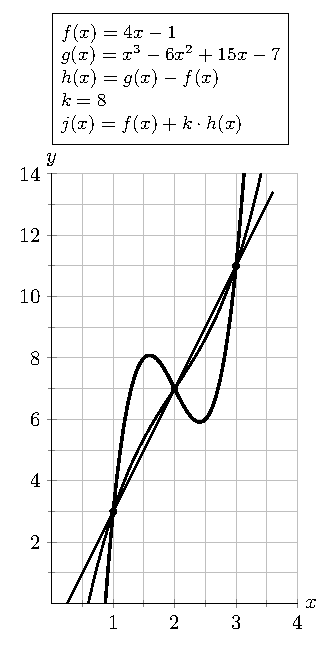
\includegraphics[width=.92\linewidth]{../figures/fhsm_2009_p39_2.pdf}
        \end{center}
    \end{scriptlist}
  }
  {
    \begin{scriptlist}
      \item [Giáo viên:] Bây giờ em có thấy mình có thể tìm một đa thức khác bằng đồ thị như thế nào không?
      
      \item [Học sinh:] Có lẽ em có thể tìm cách làm thay đổi dạng của đồ thị bậc ba nhưng vẫn giữ nguyên các giao điểm.
      
      \item [Giáo viên:] Em sẽ làm điều đó bằng đại số như thế nào?
      
      \item [Học sinh:] Em có thể thử kéo giãn hiệu giữa $f(x)$ và $g(x)$, tức là
      $$
        g(x)-f(x)=x^3-6x^2+11x-6.
      $$
      Chẳng hạn, em có thể nhân hiệu đó với $3$, rồi cộng trở lại vào $f(x)$ để được
      $$
        \begin{aligned}
          &4x-1+3(x^3-6x^2+11x-6) \\
          &\quad=3x^3-18x^2+37x-19.
        \end{aligned}
      $$

      \item [Giáo viên:] Rất tốt. Bây giờ thầy muốn hiểu điều gì thực sự đang diễn ra ở đây. Có điều gì đặc biệt ở đa thức $x^3-6x^2+11x-6$ khiến cách này hoạt động không?\vspace{\baselineskip}
      
      \item [Học sinh:] Em chưa thấy.
      
      \item [Giáo viên:] Sao em không thử phân tích nó thành nhân tử bằng CAS?
    \end{scriptlist}

    \begin{center}
      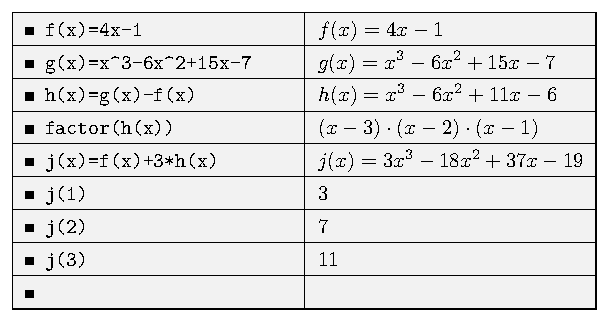
\includegraphics[width=.92\linewidth]{../figures/fhsm_2009_p39_f1.pdf}
    \end{center}

    \begin{scriptlist}  
      \item [Học sinh:] Em được
      $$
        \begin{aligned}
          &x^3-6x^2+11x-6 \\
          &\quad=(x-1)(x-2)(x-3).
        \end{aligned}
      $$

      À, em hiểu rồi. Khi nhìn dạng đã phân tích thành nhân tử, em thấy hiệu giữa $f(x)$ và $g(x)$ bằng $0$ tại $x=1,2,\text{ và }3$. Vậy nên em có thể tạo ra nhiều đa thức sinh cùng một dãy chỉ bằng cách cộng vào $f(x)$ một bội của đa thức này.

      \item [Giáo viên:] Dạng tổng quát của một đa thức như thế là gì?
      
      \item [Học sinh:] Đó là
      $$
        4x-1+k(x-1)(x-2)(x-3),
      $$
      trong đó $k$ có thể là bất kì số thực nào. Khi nhìn trên phần mềm vẽ đồ thị, em nhận thấy rằng khi $k$ tăng lên, đồ thị của đa thức càng tách xa khỏi đường thẳng.

        \begin{center}
          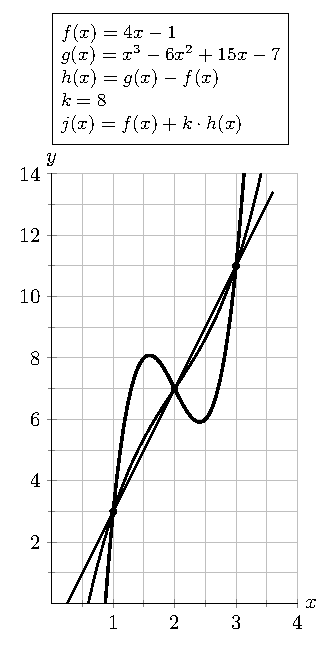
\includegraphics[width=.92\linewidth]{../figures/fhsm_2009_p39_2.pdf}
        \end{center}
    \end{scriptlist}
  }{}

\TriExampleLongNext
  {
    \textbf{Key Mathematical Elements}

    \begin{hanglist}
      \hangitem{Reasoning with Algebraic Symbols---Mindful manipulation; Linking expressions and functions}

      \hangitem{Reasoning with Functions---Using multiple representations of functions}
    \end{hanglist}

    \textbf{Reasoning Habits}

    \begin{hanglist}
      \hangitem{Analyzing a problem---identifying relevant concepts, representations, or procedures; seeking patterns and relationships}

      \hangitem{Seeking and using connections}
    \end{hanglist}
  }
  {
    \textbf{Các yếu tố then chốt của toán học}

    \begin{hanglist}
      \hangitem{Luận với kí hiệu đại số---Biến đổi có ý thức; Liên kết biểu thức và hàm số}\vspace{\baselineskip}

      \hangitem{Luận với hàm số---Sử dụng nhiều biểu diễn của hàm số}
    \end{hanglist}

    \textbf{Thói quen luận}

    \begin{hanglist}
      \hangitem{Phân tích bài toán---xác định khái niệm, thủ tục hoặc biểu diễn toán học thích đáng; tìm kiếm mẫu hình và quan hệ}

      \hangitem{Tìm kiếm và sử dụng kết nối}
    \end{hanglist}
  }{}

\CloseGrid